\documentclass[pdflatex,sn-mathphys-num]{sn-jnl}% Math and Physical Sciences Numbered Reference Style

\usepackage{graphicx}%
\usepackage{multirow}%
\usepackage{amsmath,amssymb,amsfonts}%
\usepackage{amsthm}%
\usepackage{mathrsfs}%
\usepackage[title]{appendix}%
\usepackage{xcolor}%
\usepackage{textcomp}%
\usepackage{manyfoot}%
\usepackage{booktabs}%
\usepackage{algorithm}%
\usepackage{algorithmicx}%
\usepackage{algpseudocode}%
\usepackage{listings}%
\usepackage{tikz}%
\usetikzlibrary{positioning,arrows.meta}%

\providecommand{\code}[1]{\texttt{#1}}% used in Section 4
\algrenewcommand\algorithmicrequire{\textbf{Input:}}
\algrenewcommand\algorithmicensure{\textbf{Output:}}

\theoremstyle{thmstyleone}%
\newtheorem{theorem}{Theorem}%
\newtheorem{proposition}[theorem]{Proposition}%

\theoremstyle{thmstyletwo}%
\newtheorem{example}{Example}%
\newtheorem{remark}{Remark}%

\theoremstyle{thmstylethree}%
\newtheorem{definition}{Definition}%

\raggedbottom

\begin{document}

\title[Adaptive Identification and Tracking]{Adaptive Candidate Routing for Distributed Occupant Recognition Across Multiple Building IoT-enabled Smart Spaces.}

\author*[1,2]{\fnm{First} \sur{Author}}\email{iauthor@gmail.com}

\author[2,3]{\fnm{Second} \sur{Author}}\email{iiauthor@gmail.com}
\equalcont{These authors contributed equally to this work.}

\author[1,2]{\fnm{Third} \sur{Author}}\email{iiiauthor@gmail.com}
\equalcont{These authors contributed equally to this work.}

\affil*[1]{\orgdiv{Department}, \orgname{Organization}, \orgaddress{\street{Street}, \city{City}, \postcode{100190}, \state{State}, \country{Country}}}

\affil[2]{\orgdiv{Department}, \orgname{Organization}, \orgaddress{\street{Street}, \city{City}, \postcode{10587}, \state{State}, \country{Country}}}

\affil[3]{\orgdiv{Department}, \orgname{Organization}, \orgaddress{\street{Street}, \city{City}, \postcode{610101}, \state{State}, \country{Country}}}

\abstract{In a distributed state transition system (DSTS) for multi-building camera networks, a face embedding captured in one building must be traced to the building-specific state transition system (BSTS) in which its occupant is registered, before the recognition can be translated into an event and the states updated. A centralized master gallery of face embeddings makes this easy but keeps sensitive biometric data in one place. We propose a routing strategy that avoids it. Each BSTS publishes one Bloom filter built from locality-sensitive hashing (LSH) codes of the face embeddings of its registered occupants. A captured face embedding is converted into $L$ LSH codes that are checked against all filters, and only the best-scoring BSTSs verify it against their own reference face embeddings. On 500 CASIA-WebFace identities in 10 buildings, averaged over 20 random building assignments, the default setting identifies 92.37\% of test face embeddings correctly, against 95.47\% for a centralized search with the same vote rule; an adaptive rule that asks extra BSTSs only when the ranking is unclear reaches 92.44\% and contacts 2.54 BSTSs on average. The mean face embedding and the accept angle come from reference face embeddings only; $K$ and $P$ were chosen after seeing test accuracy, so alternatives are reported. LSH code collisions raise the real false-positive rate of the filters to 3.54\% instead of the configured 1\%. When the same occupants are split over 2, 5 and 10 BSTSs, the adaptive rule stays within 0.5 points of the centralized search at 2 and 5 BSTSs (95.0\% and 95.3\% against 95.5\%) and 2.9 points below it at 10 (92.6\%), and someone who holds the filters can tell which building an occupant is registered in (AUC 0.93). \textcolor{blue}{Costs are computed, not measured; encryption and unknown individuals are not evaluated}.}

\keywords{Occupant identification and tracking, Distributed state transition system, Smart Spaces, Locality-sensitive hashing, Bloom filter, Privacy in data analytics}

\maketitle

\section{Introduction}\label{sec1}

Large camera networks that monitor several buildings can be abstracted as a distributed state transition system (DSTS), composed of independent building-specific state transition systems (BSTSs) in which recognition events drive state transitions~\cite{mohan2020}. Every occupant is registered in exactly one BSTS, and an occupant seen in another building is a visitor there. When a face embedding is captured in one building, the system must therefore find the BSTS in which its occupant is registered before the recognition can be translated into an event and the states updated. The DSTS framework resolves such visitors against a centralized master list of registered occupants~\cite{mohan2020}, that is, one central gallery with the face embeddings of everyone. This is simple and accurate, but it stores sensitive biometric data in a single place, which is an attractive target and may conflict with data-minimization rules. The other extreme is a gallery in each BSTS and a request to every BSTS for every captured face embedding, which exposes every captured face embedding to every building.

We study the step between these two: a routing step that decides which few BSTSs should be asked. Each BSTS publishes one Bloom filter~\cite{bloom1970} built from LSH codes of the face embeddings of its registered occupants. A captured face embedding is checked against all filters, and only the best-scoring BSTSs receive it. Reference face embeddings are not published. The idea of publishing a compact summary of what each site holds, and checking the summaries before contacting a site, is used in web cache sharing~\cite{fan2000}. Face matching is approximate, so the summary cannot hold exact keys; it holds LSH codes instead.

\emph{Scope.} This paper is about the routing step. We measure how accurate it is, how many BSTSs it contacts, how many false positives the filters give, and how it behaves with 2, 5 and 10 BSTSs. All evaluated face embeddings belong to registered occupants; identifying unknown individuals, who are registered in no BSTS, is left for future work. We do not implement or test any cryptographic protection. We assume that messages between BSTSs use a standard authenticated, encrypted channel, and Section~\ref{sec:model} states what is and is not protected. Storage and communication costs are computed from message sizes; no distributed run was measured.

Our contributions are:
\begin{itemize}
\item a routing design with one Bloom filter of LSH codes per BSTS, and a way to choose the code length $K$ and the number of codes $L$ from measured angle distributions;
\item measurements on 500 identities and 20 building assignments: accuracy against a centralized search, the gain from multi-probe hashing, and a real false-positive rate of 3.54\% that we trace to collisions between LSH codes;
\item a rule that asks extra BSTSs only when the two best scores are close, which is as accurate as asking all shortlisted BSTSs and contacts about half as many;
\item an evaluation with 2, 5 and 10 BSTSs, an analytic cost comparison, and a measurement of what the published filters reveal about the building in which an occupant is registered.
\end{itemize}

%=====================================================================
\section{Related Work}
\label{sec:related}
Occupant identification and tracking in smart spaces has been modelled with state transition systems whose events abstract the recognition step and whose transition function abstracts the reasoning behind state changes~\cite{MJG2011}. The DSTS extends this to multi-building camera networks as independent BSTSs, and resolves a visitor against a centralized master list of registered occupants~\cite{mohan2020}; we replace that lookup by routing. Other occupant tracking work uses RF signals~\cite{WZSYGWLLHSC2025}, camera-based surveillance analysis such as video synopsis~\cite{NGA2022}, and quantitative metrics for smart spaces~\cite{MMJ2025}. Across multi-building smart spaces, computational efficiency and privacy preservation remain the two main challenges, especially with camera-based sensing~\cite{KKZWKMW2025}. Facial biometrics suit identification in IoT-enabled smart spaces~\cite{KZGS2024} because they carry distinctive identity information and can be captured remotely, without the person stopping, cooperating, or presenting a credential.

\emph{Template protection and Bloom filters.} Rathgeb et al.~\cite{rathgeb2014} apply Bloom filters to iris templates. Closest to our work, Marzani et al.~\cite{marzani2026} turn face features into identifiers with a fuzzy extractor and store them in homomorphically encrypted Bloom filters to count people across locations. Their goal is counting by exact identifier membership; ours is routing a face embedding by approximate similarity (LSH codes with multi-probe) to the BSTS in which its occupant is registered.

\emph{Routing in distributed search.} Summary Cache~\cite{fan2000} lets web proxies exchange Bloom filters of their contents and contact only matching proxies; our routing step follows this idea with LSH codes in place of exact keys. For vector data, Gottesb{\"u}ren et al.~\cite{gottesbueren2024} study clustering- and LSH-based methods that send a search request only to shards likely to hold its neighbours. Semord~\cite{wang2026semord} places similar vectors close together in a decentralized overlay using a learned hash; its peers exchange summaries that include representative vectors, and it is evaluated on generic benchmarks, not on face embeddings or with a privacy goal. These systems route by vector placement, centroids or learned structure, which requires moving data or sharing vector summaries. We instead let each BSTS publish a small Bloom filter of LSH codes and keep its reference face embeddings. To our knowledge, the combination of LSH codes and per-BSTS Bloom filters has not been measured for this task before.

%=====================================================================
\section{Methodology}
\label{sec:method}

The method has two phases: each BSTS builds its Bloom filter once (Algorithm~\ref{alg:build}), and every captured face embedding is then routed, verified, and translated into a recognition event (Algorithm~\ref{alg:adaptive-routing}). We first state the setting and what is protected, then define the quantities that the algorithms use.

\subsection{System and Threat Model}
\label{sec:model}

We build on the distributed state transition system (DSTS) of~\cite{mohan2020} (Figure~\ref{fig:arch}), which abstracts a multi-building camera network as independent building-specific state transition systems (BSTSs). Each BSTS$_b$ has a set of states, a set of events and a transition function $\Delta^b:S^b\times E^b\to S^b$; a state records the probabilities of occupants being present in the zones of the building~\cite{mohan2020,MJG2011}. BSTS$_b$ stores the reference face embeddings of its $N$ registered occupants; an occupant registered in another BSTS is a visitor there. A face captured at event instance $k$ in a zone of building $q$ is converted into a face embedding. Recognition of this face embedding is translated into a recognition event $e_k$, and the transition function derives the next state $S_k$ from the current state $S_{k-1}$. When the occupant is registered in another BSTS, the DSTS looks the face embedding up in a centralized master list of all registered occupants~\cite{mohan2020}; this paper replaces that lookup by the routing step below and evaluates the identification step only. We assume that every occupant is registered in exactly one BSTS. Each BSTS constructs a Bloom filter from the Locality-Sensitive Hashing (LSH) codes of the face embeddings of its registered occupants, and the system uses these filters to shortlist candidate BSTSs, which verify the captured face embedding against their stored reference face embeddings. Reference face embeddings are not exchanged between BSTSs during routing or verification, although the captured face embedding is sent to shortlisted BSTSs. We assume that BSTSs execute these operations correctly but may attempt to infer sensitive information from received data. Published Bloom filters, public hash parameters and captured face embeddings may reveal building membership, as evaluated in Section~\ref{sec:leak}. Authenticated and encrypted communication is assumed but not implemented or evaluated. Candidate-face guessing, external information, repeated captures, colluding BSTSs, malicious behavior, and traffic analysis are outside the scope of this study.

\begin{figure}[!t]
\centering
\small
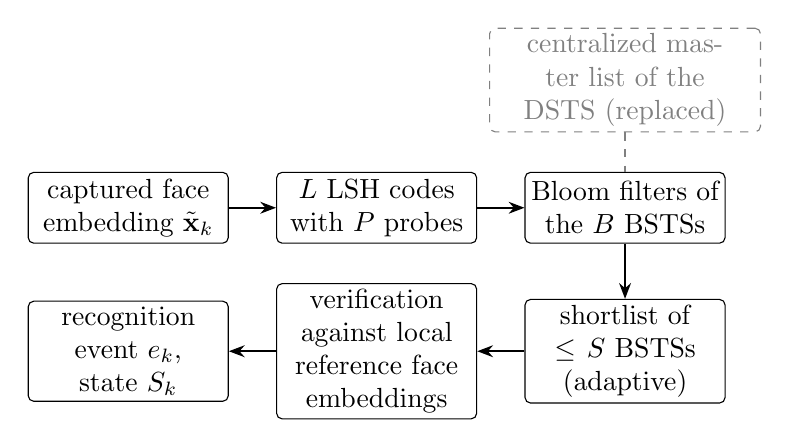
\begin{tikzpicture}[
  box/.style={draw, rounded corners=2pt, align=center, minimum height=9mm, text width=24mm, inner sep=2pt},
  gal/.style={draw, dashed, gray, rounded corners=2pt, align=center, text width=33mm, inner sep=2pt},
  arr/.style={-{Stealth[length=2mm]}, thick}]
  \node[box] (a) {captured face embedding $\tilde{\mathbf{x}}_k$};
  \node[box, right=6mm of a] (b) {$L$ LSH codes with $P$ probes};
  \node[box, right=6mm of b] (c) {Bloom filters of the $B$ BSTSs};
  \node[gal, above=5mm of c] (m) {\textcolor{gray}{centralized master list of the DSTS (replaced)}};
  \node[box, below=7mm of c] (d) {shortlist of $\le S$ BSTSs (adaptive)};
  \node[box, left=6mm of d] (e) {verification against local reference face embeddings};
  \node[box, left=6mm of e] (f) {recognition event $e_k$, state $S_k$};
  \draw[arr] (a)--(b); \draw[arr] (b)--(c); \draw[arr] (c)--(d); \draw[arr] (d)--(e); \draw[arr] (e)--(f);
  \draw[gray, dashed] (m)--(c);
\end{tikzpicture}
\caption{Routing in a DSTS. A captured face embedding is checked against the published Bloom filter of every BSTS, only the shortlisted BSTSs verify it with their private reference face embeddings, and the result is translated into a recognition event that updates the state.}
\label{fig:arch}
\end{figure}

\subsection{Face Embedding and LSH Codes}
For the face $o_k$ captured at event instance $k$, SCRFD-10GF~\cite{guo2022} detects the face and pretrained ArcFace (InsightFace \code{buffalo\_l})~\cite{deng2019} produces a 512-dimensional raw face embedding $\tilde{\mathbf{x}}_k$; reference face embeddings are produced in the same way. We first unit-normalize and then subtract the reference-only population mean $\bar{\mathbf{x}}$ and renormalize, giving the face embedding $\mathbf{p}$ used for routing:
\begin{equation}
\mathbf{x}_k=\frac{\tilde{\mathbf{x}}_k}{\|\tilde{\mathbf{x}}_k\|_2},\qquad
\mathbf{p}=\frac{\mathbf{x}_k-\bar{\mathbf{x}}}{\|\mathbf{x}_k-\bar{\mathbf{x}}\|_2}.
\label{eq:preprocess}
\end{equation}
The same mean and transformation are used for enrollment and identification. Let $K$ be the number of bits per code and $L$ the number of slots. Using $KL$ fixed-seed Gaussian hyperplanes $\mathbf{h}_{\ell,i}$, define $b_{\ell,i}=\mathbb{1}[\mathbf{p}\cdot\mathbf{h}_{\ell,i}\geq0]$ and the slot-tagged item
\begin{equation}
c_\ell=\sum_{i=0}^{K-1}b_{\ell,i}2^i,\qquad s_\ell=\ell2^K+c_\ell.
\label{eq:lsh-code}
\end{equation}
For angle $\theta$ between two unit face embeddings, a bit matches with probability $p_{\rm bit}=1-\theta/180$~\cite{charikar2002}.

\subsection{Parameter Selection}
Averaging $p_{\rm bit}^K$ over reference-only genuine and impostor pairs of face embeddings gives $p_{\rm code}^{(G)}$ and $p_{\rm code}^{(I)}$. Assuming independent slots,
\begin{equation}
\mathrm{Recall}=1-(1-p_{\rm code}^{(G)})^L,\quad
\mathrm{FPR}_{\rm imp}=1-(1-p_{\rm code}^{(I)})^L.
\label{eq:lsh-recall}
\end{equation}
For a recall target $\rho$, set $L=\left\lceil\ln(1-\rho)/\ln(1-p_{\rm code}^{(G)})\right\rceil$. For each candidate $K$ we compute $L$, reject values with predicted $\mathrm{FPR}_{\rm imp}>\varphi$ for a chosen bound $\varphi$, and keep the pair with the smallest $KL$.

\subsection{Per-BSTS Bloom Filters}
Each BSTS publishes a Bloom filter but retains its reference face embeddings. For registered occupant $u$ in BSTS$_b$, the normalized mean of the $R$ reference face embeddings forms centroid $\mathbf{z}_{b,u}=\operatorname{Normalize}(R^{-1}\sum_{r=1}^{R}\mathbf{e}_{b,u,r})$, which is encoded into $L$ items using Equation~\ref{eq:lsh-code}. With $n=NL$ inserted items and target false-positive probability $f^\star$, the filter size and number of hash positions are
\begin{equation}
m=\left\lceil\frac{-n\ln f^\star}{(\ln2)^2}\right\rceil,\qquad
\kappa=\operatorname{round}\!\left(\frac{m}{n}\ln2\right).
\label{eq:bloom-size}
\end{equation}
We use Kirsch--Mitzenmacher double hashing~\cite{kirsch2006}: $h_1=\mathrm{SM64}(s\oplus(2\sigma+1))$, $h_2=\mathrm{SM64}(s\oplus(2\sigma+2))\vee1$, and $p_j=((h_1+jh_2)\bmod2^{64})\bmod m$ for $j=0,\ldots,\kappa-1$, where $\sigma$ is a shared salt and SM64 is the SplitMix64 finalizer~\cite{steele2014}. A check is positive when all $\kappa$ positions are set.

\begin{algorithm}[!t]
\small
\caption{Building the published Bloom filter at BSTS$_b$}
\label{alg:build}
\begin{algorithmic}[1]
\Require Raw reference face embeddings $\tilde{\mathbf{x}}_{b,u,r}$ of the $N$ registered occupants of BSTS$_b$ ($R$ per occupant);
\Statex population mean $\bar{\mathbf{x}}$; shared hyperplanes $\mathcal{H}$ and salt $\sigma$; parameters $K,L,f^\star$.
\Ensure Published Bloom filter $F_b$; private reference face embeddings $\mathcal{E}_b$.
\State $n\gets NL$; derive $m$ and $\kappa$ \Comment{Equation~\ref{eq:bloom-size}}
\State $F_b\gets$ all-zero bit array of length $m$
\For{$u=1$ to $N$}
  \For{$r=1$ to $R$}
    \State $\mathbf{e}_{b,u,r}\gets$ preprocessed $\tilde{\mathbf{x}}_{b,u,r}$ \Comment{Equation~\ref{eq:preprocess}}
  \EndFor
  \State $\mathbf{z}_{b,u}\gets\operatorname{Normalize}\bigl(R^{-1}\sum_{r}\mathbf{e}_{b,u,r}\bigr)$ \Comment{occupant centroid}
  \For{$\ell=0$ to $L-1$}
    \State $s_\ell\gets$ slot-tagged item of $\mathbf{z}_{b,u}$ \Comment{Equation~\ref{eq:lsh-code}}
    \State set the $\kappa$ bits $p_0,\dots,p_{\kappa-1}$ of item $s_\ell$ in $F_b$ \Comment{double hashing}
  \EndFor
\EndFor
\State $\mathcal{E}_b\gets\{\mathbf{e}_{b,u,r}\}$, kept private; publish $F_b$
\end{algorithmic}
\end{algorithm}

\subsection{Routing, Verification, and Event Generation}\label{sec:escalation}
For each slot, multi-probe routing~\cite{lv2007} checks the original code and $P$ single-bit variants obtained by flipping the bits with the smallest margins $|\mathbf{p}\cdot\mathbf{h}_{\ell,i}|$:
\begin{equation}
s'_{\ell,j}=\ell2^K+\bigl(c_\ell\mathbin{\mathrm{XOR}}2^{w_{\ell,j}}\bigr),\quad j=1,\ldots,P,
\label{eq:multi-probe}
\end{equation}
where $w_{\ell,j}$ is the index of the $j$-th smallest-margin bit. BSTS$_b$ receives score $A_b$, the number of slots with at least one positive check; the shortlist $\mathcal{C}$ contains the top $\min(S,B)$ BSTSs by score (ties by index). In a shortlisted BSTS, each reference face embedding votes for its registered occupant when its angle to the captured face embedding is at most the accept angle $\tau$, the cutoff that minimizes the sum of the genuine false-reject rate and the impostor false-accept rate on reference face embeddings; the local winner is the registered occupant with most votes (ties by smallest reference angle), and acceptance requires at least $V$ of $R$ votes. The adaptive policy verifies all shortlisted BSTSs when $g=A_{(1)}-A_{(2)}\leq g_0$ and selects by vote count, minimum reference angle, then routing rank; otherwise it stops at the first local acceptance in routing order. An accepted occupant is translated into the recognition event $e_k$ of the BSTS in which it is registered, and the transition function updates the state. If none is accepted, the system abstains, no event is generated and the state is left unchanged. The default all-shortlist rule used in the multi-probe comparison instead compares votes across all registered occupants of the shortlisted BSTSs, breaking ties by minimum reference angle.

\begin{algorithm}[!t]
\small
\caption{Adaptive candidate routing, event generation and state generation}
\label{alg:adaptive-routing}
\begin{algorithmic}[1]
\Require Face embedding $\tilde{\mathbf{x}}_k$ captured at event instance $k$ in zone $j$ of building $q$;
\Statex published filters $\{F_b\}_{b=1}^{B}$; private reference face embeddings $\{\mathcal{E}_b\}_{b=1}^{B}$ held by the BSTSs;
\Statex mean $\bar{\mathbf{x}}$, hyperplanes $\mathcal{H}$, parameters $K,L,P,S,V,\tau,g_0$;
\Statex current state $S_{k-1}$.
\Ensure Recognised occupant $a^\star$ registered in BSTS$_{b^\star}$ (or $\mathrm{ABSTAIN}$), event $e_k$ and next state $S_k$.
\State $\mathbf{p}\gets$ preprocessed $\tilde{\mathbf{x}}_k$ \Comment{Equation~\ref{eq:preprocess}}
\For{$\ell=0$ to $L-1$}
  \State compute $s_\ell$ and the $P$ probe items $s'_{\ell,1},\dots,s'_{\ell,P}$ \Comment{Eqs.~\ref{eq:lsh-code}, \ref{eq:multi-probe}}
\EndFor
\For{$b=1$ to $B$}
  \State check the original and probe items of every slot against $F_b$
  \State $A_b\gets$ number of slots with at least one positive check \Comment{each slot once}
\EndFor
\State $\mathcal{C}\gets$ top $\min(S,B)$ BSTSs by decreasing $A_b$ \Comment{ties by index}
\State $g\gets A_{(1)}-A_{(2)}$ if $B\geq2$, else $g\gets+\infty$
\State $a^\star\gets\mathrm{ABSTAIN}$
\If{$g\leq g_0$} \Comment{ranking unclear: verify all shortlisted BSTSs}
  \ForAll{$b\in\mathcal{C}$}
    \State $(u_b,v_b)\gets\textsc{LocalVerify}(b,\mathbf{p})$
  \EndFor
  \State $\mathcal{A}\gets\{b\in\mathcal{C}:v_b\geq V\}$
  \If{$\mathcal{A}\neq\emptyset$} \State $(a^\star,b^\star)\gets(u_b,b)$ for the $b\in\mathcal{A}$ with most votes \Comment{ties: angle, then rank} \EndIf
\Else \Comment{ranking clear: sequential first-match}
  \ForAll{$b\in\mathcal{C}$ in routing order}
    \State $(u_b,v_b)\gets\textsc{LocalVerify}(b,\mathbf{p})$
    \If{$v_b\geq V$} \State $(a^\star,b^\star)\gets(u_b,b)$; \textbf{break} \EndIf
  \EndFor
\EndIf
\State $e_k\gets\textit{event\_gen}(a^\star,b^\star,k,q,j)$ \Comment{recognition translated into an event; none on $\mathrm{ABSTAIN}$}
\State $S_k\gets\textit{state\_gen}(S_{k-1},e_k)$ \Comment{transition function $\Delta$; $S_k=S_{k-1}$ on $\mathrm{ABSTAIN}$}
\State \Return $a^\star,e_k,S_k$
\Function{LocalVerify}{$b,\mathbf{p}$} \Comment{runs in BSTS$_b$ on its private reference face embeddings}
  \ForAll{registered occupant $u$ of BSTS$_b$}
    \State $v_u\gets|\{r:\angle(\mathbf{p},\mathbf{e}_{b,u,r})\leq\tau\}|$
  \EndFor
  \State \Return $u^\star=\arg\max_u v_u$ (ties by smallest reference angle) and $v_{u^\star}$
\EndFunction
\end{algorithmic}
\end{algorithm}

\section{Experimental Setup}
\label{sec:setup}

We use the face embeddings of 500 identities of CASIA-WebFace~\cite{yi2014}, registered in $B=10$ BSTSs of $N=50$ occupants each. Each occupant has $R=20$ reference face embeddings and 20 held-out test face embeddings, giving 20,000 face embeddings. Every one of the 10,000 test face embeddings is processed as one event instance: it is routed over all $B$ BSTSs and its recognition is translated into an event. The evaluation is \emph{closed-set}: every test face embedding belongs to an occupant registered in exactly one BSTS. We use $K=11$, $L=122$, $P=3$, $S=5$, $V=12$ and $f^{\star}=0.01$. With these settings each filter stores $n=NL=6{,}100$ items and has $m=58{,}469$ bits and $\kappa=7$ hash positions (about 7.3\,KB). For parameter selection (Section~\ref{sec:method}) we use a recall target $\rho=0.90$, an impostor-FPR bound $\varphi=0.10$ and $K\in\{4,\ldots,15\}$; the model selects $(K,L)=(10,88)$, whereas the main experiments use $(11,122)$ because it performed better on test accuracy (Section~\ref{sec:k1011}).

\emph{Use of test data.} The mean face embedding, the accept angle and the angle statistics behind $K$ and $L$ are estimated from reference face embeddings only: the mean is taken over the 10,000 reference face embeddings, genuine pairs are two reference face embeddings of the same occupant, and impostor pairs are reference face embeddings of different occupants. This gives $\tau=80.43^{\circ}$. An earlier version used test face embeddings for the mean and $\tau$ ($80.54^{\circ}$); with reference-only estimates, correct-identification rates changed by at most 0.06 points, and misidentification rates fell by 0.1 to 0.15 points. Since $K=11$ and $P=3$ were chosen after looking at test accuracy, we also report $K=10$, the model's choice, and the full sweep over $P$ (Section~\ref{sec:k1011}).

\emph{Seeds.} Each result is repeated for 20 seeds. A seed changes three things together: the assignment of the 500 identities to BSTSs of 50 registered occupants, the LSH hyperplanes, and the Bloom filter salt. The face embeddings, their mean and the accept angle stay fixed, so the centralized baseline is a single number. We report the mean over seeds with a 95\% confidence half-width ($\pm$, Student-$t$, 19 degrees of freedom) and, for comparisons, the paired difference over seeds. For $B=2$ and $B=5$, we regroup the occupants of the first two and first five buildings of the original layout into BSTSs of 50. A single run with the original assignment and hyperplane seed 42 gave 92.32\% at $P=3$ with the default rule, 0.05 points below the 20-seed mean.

\emph{Metrics.} Each test face embedding results in exactly one of four recognition outcomes: \emph{correct} (the event names the right registered occupant); \emph{misidentified} (a wrong occupant is accepted, the most serious error); \emph{abstained-reject} (the true BSTS was shortlisted but nobody reached $V$ votes); and \emph{abstained-routing} (the true BSTS was not shortlisted and nobody reached $V$ votes). The centralized baseline gives 95.47\% correct, 1.41\% misidentified and 3.12\% abstained.

%=====================================================================
\section{Results}
\label{sec:results}

\subsection{Choice of $K$ and $L$}
\label{sec:k1011}

The analytic model uses only the angle arrays, so it has no seed. Using the mean angle first gives
$p_{\text{code}}^{(G)}=0.0115$ at $K=11$, against the correct array average of $0.0187$, which is about
39\% too low. The model picks $K=10$, $L=88$. In the full pipeline at $P=3$ with the default rule, $K=11$,
$L=122$ is more accurate than $K=10$ by $0.52 \pm 0.13$ points (paired) and better in 20 of 20 seeds: correct
92.37\% against 91.85\%, mainly because routing failures fall from 4.88\% to 4.46\%. Both results are reported; we use
$K=11$ in the rest of the paper, and we note that this choice was made after seeing test accuracy.

\subsection{Multi-Probe and Decentralized versus Centralized Identification}

Table~\ref{tab:probe} varies $P$ at $B=10$ with the default rule. Without probing, $8.07 \pm 0.11\%$ of face embeddings are lost
to routing misses. Multi-probe with $P=3$ reduces this to $4.46 \pm 0.08\%$ (a 45\% relative reduction), raises
correct identification from $88.28\%$ to $92.37\%$ (a paired gain of $4.09 \pm 0.15$ points, positive in
20 of 20 seeds) and lowers misidentification from 1.91\% to 1.42\%. The gains get smaller as $P$
grows, while the number of lookups grows linearly, so we use $P=3$ as a compromise on cost, not as the best possible
value.

\begin{table}[!t]
\caption{Multi-probe sweep at $B=10$ ($K=11$, $L=122$, default rule).
Results are reported as the mean over 20 seeds ($\pm$ 95\% CI), in \%.
The number of items looked up per filter and face embedding is $L(1+P)$.}
\label{tab:probe}

\begin{tabular*}{\textwidth}
{@{\extracolsep\fill}cccccc}
\toprule
$P$
& Correct & Misid. & Abst.-reject & Abst.-routing & Items \\
\midrule

0 & $88.28 \pm 0.13$ & $1.91 \pm 0.04$ & $1.74 \pm 0.03$ & $8.07 \pm 0.11$ & 122 \\

1 & $90.92 \pm 0.09$ & $1.61 \pm 0.04$ & $1.71 \pm 0.04$ & $5.76 \pm 0.11$ & 244 \\

2 & $91.90 \pm 0.09$ & $1.45 \pm 0.04$ & $1.73 \pm 0.05$ & $4.92 \pm 0.10$ & 366 \\

3 & $92.37 \pm 0.08$ & $1.42 \pm 0.03$ & $1.75 \pm 0.04$ & $4.46 \pm 0.08$ & 488 \\

5 & $92.80 \pm 0.07$ & $1.38 \pm 0.03$ & $1.77 \pm 0.05$ & $4.05 \pm 0.07$ & 732 \\

7 & $92.89 \pm 0.07$ & $1.38 \pm 0.03$ & $1.76 \pm 0.05$ & $3.97 \pm 0.08$ & 976 \\
\botrule
\end{tabular*}

\end{table}

\noindent We now compare the decentralized system with the centralized baseline. At $B=2$ and $B=5$ the shortlist of
$S=5$ covers every BSTS, so routing cannot fail and the two systems give the same result in every seed
(95.75\% correct at $B=2$ and 95.64\% at $B=5$). At $B=10$ the decentralized system is $3.10 \pm 0.08$ points behind the
baseline, and 4.46\% of face embeddings are routing failures. Before multi-probe the gap was 7.19 points, so
multi-probe closes 57\% of it. Misidentification (1.42\% against 1.41\%) hardly changes, so the
loss comes from missed matches and not from more wrong accepts.

\subsection{Effective False-Positive Rate}
\label{sec:fpr}

The 1\% target describes the bit array for items that are independent of the stored ones. We measured the rate the
system really has by building all ten filters and testing the enrolled items of the \emph{other nine} BSTSs
against each one. The real per-item rate is $3.54 \pm 0.02\%$ over the 20 seeds. When we compare the integer codes
directly, without a Bloom array, $2.61 \pm 0.02\%$ of the items of other BSTSs already equal an enrolled item in the
same slot. This is close to the 2.41\% expected if the codes of 50 registered occupants were evenly spread over
$2^{11}=2048$ values, namely $1-(1-2^{-K})^{N}$. The Bloom array alone, tested on random integers that were never
inserted, gives $0.94 \pm 0.01\%$ at 51.3\% fill, close to its design rate. The extra false positives therefore come
from the LSH codes, not from the Bloom array.

A larger $K$ gives more possible codes and lowers the real false-positive rate, but $L$ must grow to keep recall at
0.90. At $K=13$, $L=230$ each filter grows from 7.3\,KB to about 13.8\,KB and the real rate falls to
1.67\%. With $P=6$ it is $0.21 \pm 0.08$ points more accurate than the best $K=11$ setting ($P=7$,
92.89\%; paired, better in 19 of 20 seeds) and $0.73 \pm 0.11$ points more accurate than the
default (93.10\% against 92.37\%; better in 20 of 20 seeds), but it needs 1,610 lookups
per filter and face embedding against 488 or 976.

\subsection{Verification Policies}
\label{sec:adaptive}

Figure~\ref{fig:results}(a) shows the policies of Section~\ref{sec:escalation} and the fixed shortlist sizes; the figures in this paragraph are the 10,000 test face embeddings of the main experiment. These
results use the policies' own rule for choosing among BSTSs (best registered occupant per BSTS, ties by rank order), so
verify-all gives 92.34\% here and not the 92.37\% of the default rule in Table~\ref{tab:probe}. The two differ
only when two shortlisted BSTSs return the same number of votes, which happens for 72.5 of 10,000 face embeddings on
average. Each captured face embedding is scored against all ten filters, including that of the occupant's home BSTS, so there is no separate local-recognition
stage. Sequential first-match raises the misidentification rate to 2.17\%, because a wrong BSTS ranked above
the true one sometimes confirms first. Asking all five BSTSs lowers it to 1.45\% and gains $0.71 \pm 0.03$ points,
but it contacts 5 BSTSs per face embedding. The adaptive rule with $g_0=5$ is slightly more accurate than asking all
five ($+0.10 \pm 0.02$ points, paired, better in 20 of 20 seeds) while contacting 2.54 BSTSs on average;
37.6\% of the face embeddings ask all five. All three policies abstain on exactly the same face embeddings, because acceptance
depends only on whether some shortlisted BSTS reaches $V$ votes.


\subsection{Cost}
\label{sec:cost}

Costs are computed from message sizes and the measured number of BSTSs asked; they are not measured in a distributed run, because all calls were in-process. A face embedding has 512 single-precision values (2,048 bytes). Routing replaces a 20.5\,MB master gallery in one place with ten published filters of 7.3\,KB each (the BSTSs keep 2.05\,MB of private reference face embeddings each). Handling one captured face embedding costs 3.1\,KB with sequential asking (1.50 BSTSs), 5.2\,KB with the adaptive rule (2.54 BSTSs) and 10.2\,KB when all five shortlisted BSTSs are asked, against 20.5\,KB for all ten BSTSs and 2.0\,KB for a master gallery. Each face embedding still needs $B\cdot L(1+P)=4{,}880$ filter lookups, which grow linearly with $B$.

\subsection{What the Filters Reveal}
\label{sec:leak}

We measured the simplest attack. Someone who holds all published filters and the public hash parameters scores a
face embedding against every filter, in the same way as routing does. With $P=3$, this score separates the registered occupants of a
BSTS from everyone else with an AUC of 0.93 (0.88 without probing), averaged over BSTSs and
10 seeds, and the highest-scoring BSTS is the occupant's own for 79.7\% of the face embeddings
(66.7\% without probing). The filters therefore leak which building an occupant is registered in. This is not a way to
recover a face, but it is a real leak, and it grows with the accuracy of the routing itself. We did not test attacks
that use many face embeddings, candidate guessing or outside information, so we make no claim of biometric privacy.

\subsection{Fewer and More BSTSs}
\label{sec:scale}

The corpus has 500 identities, so we split the same 500 registered occupants over $B=2$, 5 and 10 BSTSs of 250, 100 and 50 occupants. Each filter is sized for its own number of occupants. We use 2,000 test face embeddings per seed (4 per occupant) and 10 seeds; this subset gives 92.6\% for the adaptive rule at $B=10$, against 92.44\% on all 10,000 face embeddings. The shortlist holds at most $S=\min(5,B)$ BSTSs, so at $B=5$ it covers every BSTS (recall 100\%), and Figure~\ref{fig:results}(b) therefore reports recall for a shortlist of two. That recall falls from 100\% at $B=2$ to 89.6\% at $B=5$ and 87.0\% at $B=10$, because the shortlist is a smaller share of the BSTSs. Correct identification with the adaptive rule is 95.0\% and 95.3\% at $B=2$ and 5, close to the 95.5\% of the centralized search, and 92.6\% at $B=10$, where the adaptive rule contacts 2.5 BSTSs. The loss at $B=10$ comes from choosing among more BSTSs, not from more false hits per filter.

\begin{figure}[!t]
\centering
\includegraphics[width=\textwidth]{results_plots}
\caption{(a) Correct identification against the number of BSTSs contacted at $B=10$: fixed shortlist of $s$ BSTSs, sequential first-match, the adaptive rule and the centralized search. (b) Recall of a shortlist of two and correct identification (adaptive rule and centralized search) for 2, 5 and 10 BSTSs. Mean over 10 seeds with 95\% intervals; 2,000 test face embeddings per seed.}
\label{fig:results}
\end{figure}

%=====================================================================
\section{Limitations and Conclusion}
\label{sec:limits}

\emph{Limitations.} All results use the same 500 identities from one public dataset; the intervals reflect building assignments and hash randomness, not a different population. The values $K=11$ and $P=3$ were chosen after seeing test accuracy, and we report alternatives next to them. CASIA-WebFace data come from the web, not from deployed camera networks, so real accuracy is probably lower, and we did not check how much the training data of the pretrained ArcFace model overlaps with CASIA-WebFace. The largest network has 10 BSTSs of 50 registered occupants. The evaluation is closed-set; a first test with held-out identities showed that the vote rule ($\tau$ and $V=12$) can accept a noticeable share of them, so it must be tightened before unknown individuals are handled. We evaluated the identification step only, not the generated events, the mapping of recognition scores to occupant-presence probabilities, or the state updates over a sequence of events. Costs are computed from message sizes, not measured in a distributed run. We did not implement or evaluate the encrypted channel, visit-length template storage, or attacks beyond the membership test of Section~\ref{sec:leak}. A Bloom filter cannot delete items, so a change in registration needs a rebuild.

\emph{Conclusion.} Per-BSTS Bloom filters of LSH codes can route captured face embeddings to the BSTS of the registered occupant without a centralized master gallery. With multi-probe hashing the default setting identifies 92.37\% of test face embeddings correctly at 10
buildings against 95.47\% for a centralized search, and the adaptive rule reaches 92.44\% while contacting
about 2.54 BSTSs. The cost is lost recall that grows with the number of BSTSs, and a false-positive
rate that LSH collisions raise well above the Bloom filter's design value. The privacy conclusions are limited to what
was evaluated: the design avoids publishing reference face embeddings and a master gallery, and it leaks which building an
occupant is registered in (AUC 0.93); encryption, stronger attacks and template storage during visits were not
evaluated. The next steps are a larger and more varied population, the identification of unknown individuals with a
stricter acceptance rule, and measurements of event generation and state updates over event sequences in a distributed deployment.

\backmatter

\bmhead{Acknowledgement}

The authors gratefully acknowledge Sri Mata Amritanandamayi Devi (Amma), Chancellor, Amrita Vishwa Vidyapeetham, for her inspiration and for providing financial support for the Article Processing Charges (APC) of this publication.

\bibliography{akd}% akd.bib

\end{document}
